\chapter{Experimental Setup}
\section{X-ray tube}
\begin{figure}[H]
    \centering
    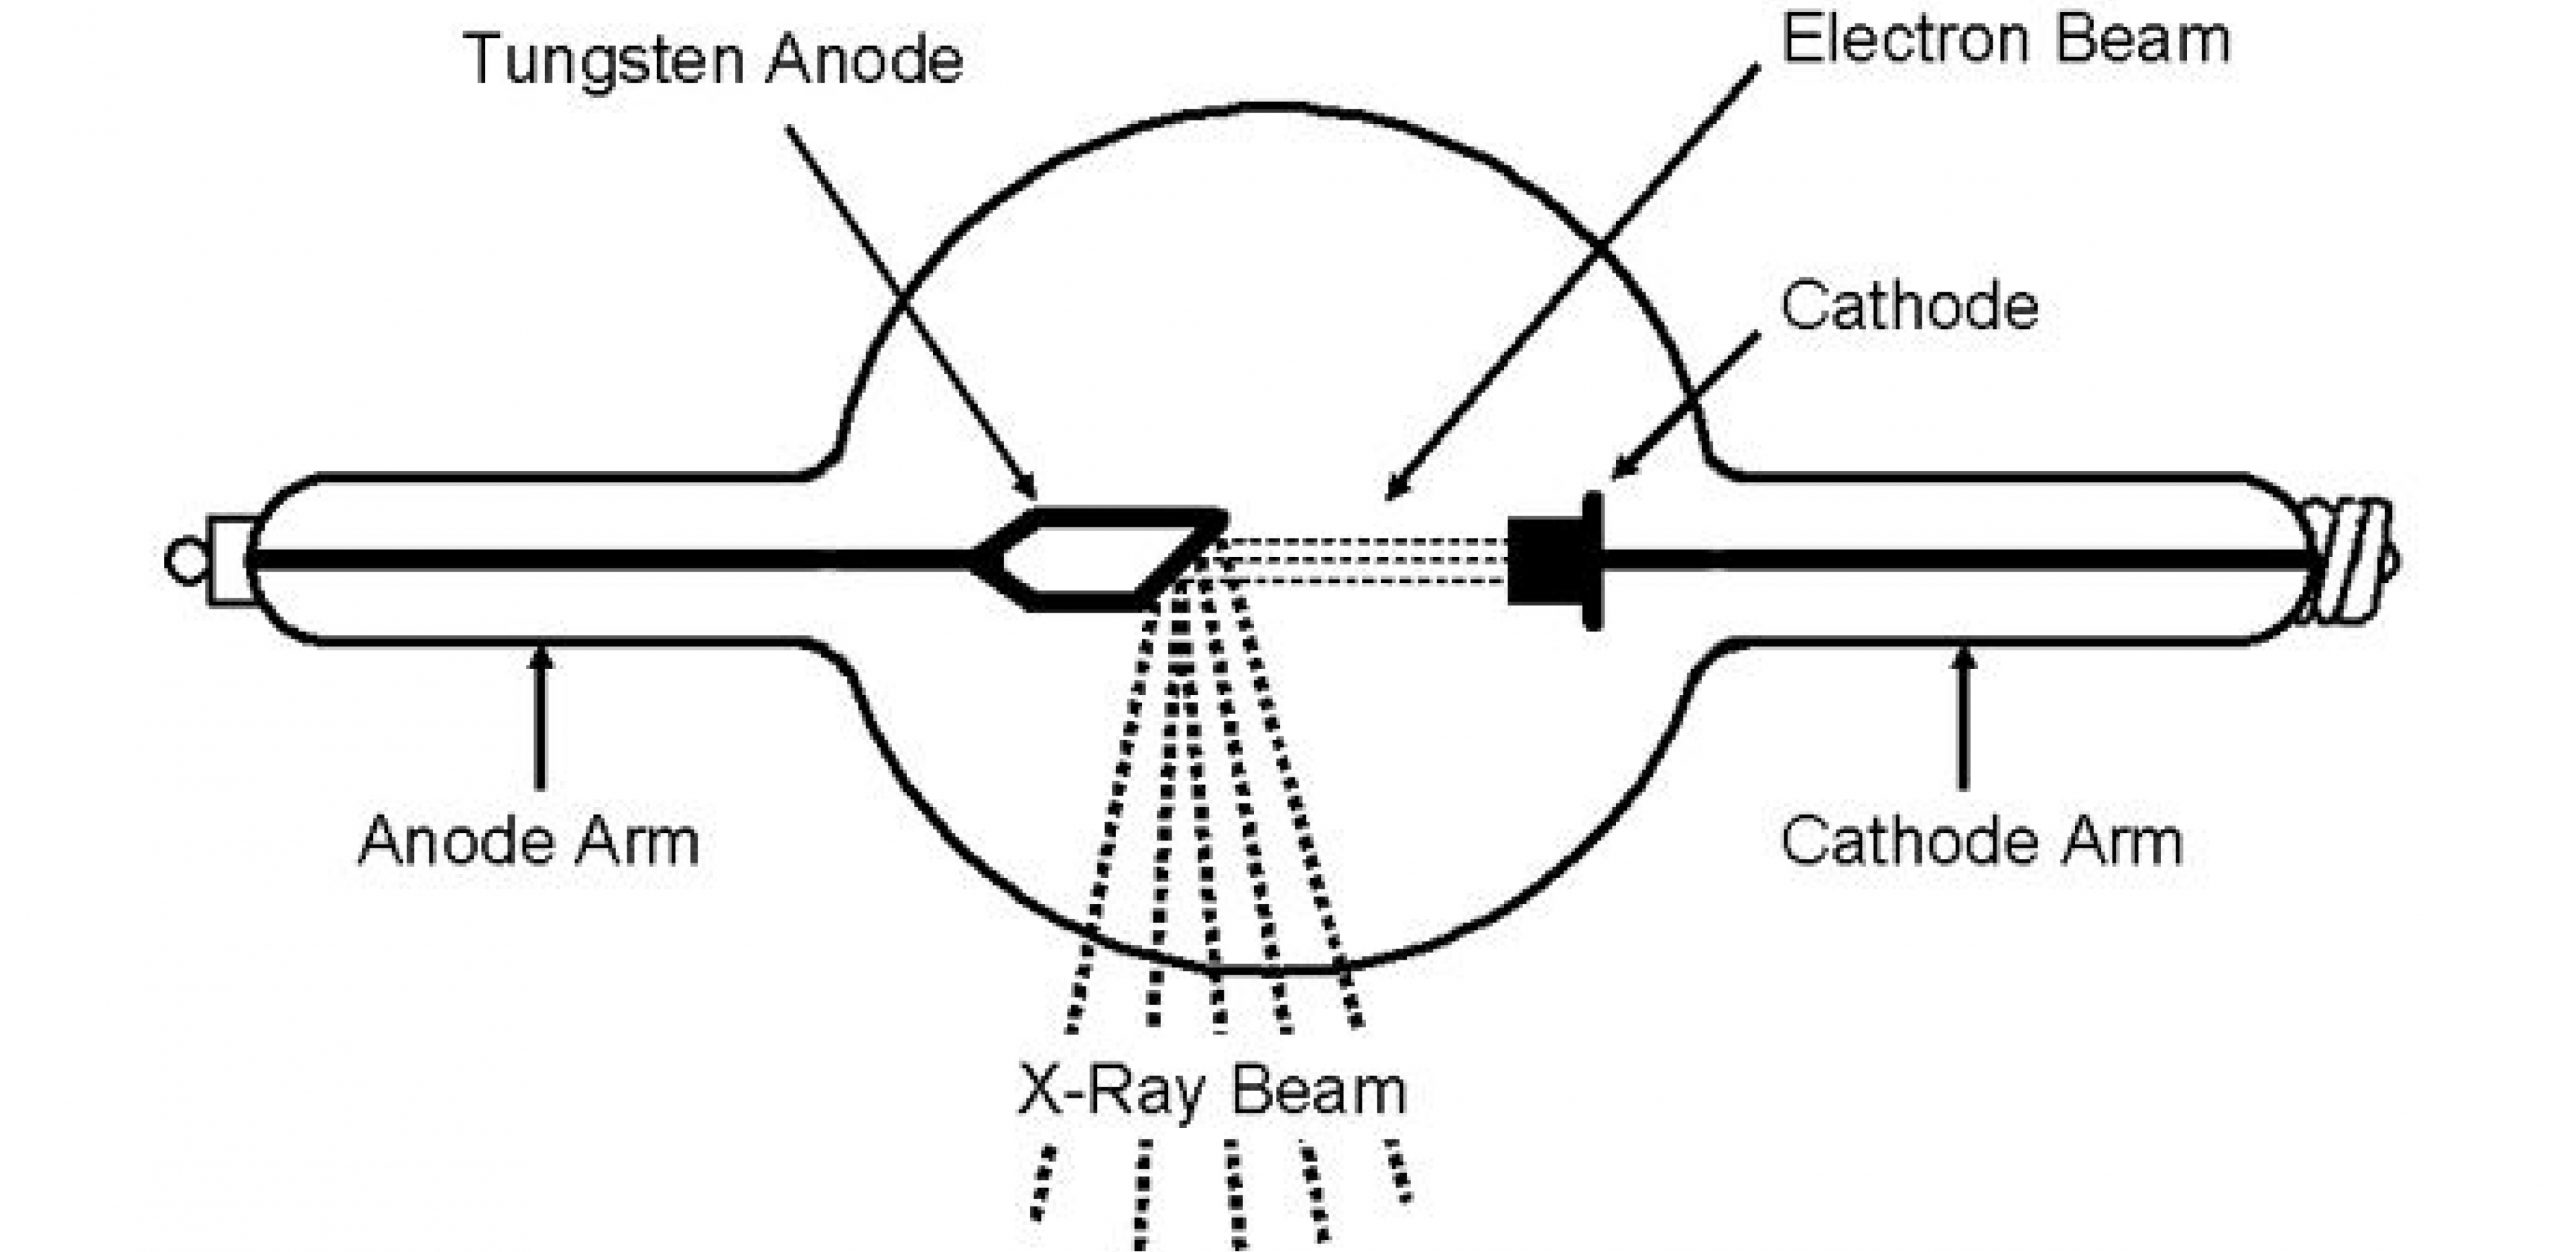
\includegraphics[width=80mm,scale=0.35]{MAX/include/X-ray tube.PNG}
    \caption{X-ray tube}
    \label{fig:X-ray tube}
\end{figure}
In the tube, there is a heated cathode that emits electrons. Due to the high voltage power source connecting the cathode and the anode, the electrons are accelerated to the anode. When the electrons collide with the material of the anode, for which tungsten is often used, they interact with electrons of tungsten nuclei. Only about $1\,\%$ of the energy generated is emitted as X-rays, whereas the rest of the energy is transformed into heat.

\section{Semiconductor detector}
Semiconductor detectors are used for the detection of ionized radiation. They have a diode, on which DC voltage is applied on in reverse bias, hence there is no current. When radiation hits the diode material, it produces free electrons and electron-holes. Due to an electric field, they travel to the electrodes as charge carriers, where they can be measured as a current pulse. Measuring the number of electron-hole pairs, so the current pulses, allows the energy of the incident radiation to be determined.


\section{Multichannel analyzer}
A multichannel analyzer is an instrument to analyze an input signal consisting of voltage pulses. It records incoming pulses and can store information about the pulses. It classifies the incoming voltage pulses according to their pulse height by assigning a value interval for the pulse heights to a channel. Hence, a channel contains the number of registered voltage signals whose pulse height lies within the interval of the channel.